\subsection{Vocal Call Locator (VCL)}
{{\footnotesize
\noindent The first large-scale benchmark (767K sounds across 9 conditions) for localizing rodent vocal calls using synchronized audio and video in standard lab environments, enabling systematic evaluation of sound-source localization algorithms in bioacoustics .


\begin{description}[labelwidth=4cm, labelsep=1em, leftmargin=4cm, itemsep=0.1em, parsep=0em]
  \item[date:] 2024-12-13
  \item[version:] v1.0
  \item[last\_updated:] 2024-12
  \item[expired:] unknown
  \item[valid:] yes
  \item[valid\_date:] 2024-12-13
  \item[url:] \href{https://neurips.cc/virtual/2024/poster/97470}{https://neurips.cc/virtual/2024/poster/97470}
  \item[doi:] unknown
  \item[domain:] Neuroscience; Bioacoustics
  \item[focus:] Benchmarking sound-source localization of rodent vocalizations from multi-channel audio
  \item[keywords:]
    - source localization
    - bioacoustics
    - time-series
    - SSL
  \item[licensing:] unknown
  \item[task\_types:]
    - Sound source localization
  \item[ai\_capability\_measured:]
    - Source localization accuracy in bioacoustic settings
  \item[metrics:]
    - Localization error (cm)
    - Recall/Precision
  \item[models:]
    - CNN-based SSL models
  \item[ml\_motif:]
    - Real-time
  \item[type:] Dataset
  \item[ml\_task:]
    - Anomaly detection / localization
  \item[solutions:] 0
  \item[notes:] Dataset spans real, simulated, and mixed audio; supports benchmarking across data types .

  \item[contact.name:] Ralph Peterson
  \item[contact.email:] unknown
  \item[results.links.name:] ChatGPT LLM
  \item[fair.reproducible:] Yes
  \item[fair.benchmark\_ready:] Yes
  \item[id:] vocal\_call\_locator\_vcl
  \item[Citations:] \cite{neurips2024_c00d37d6}
\end{description}

{\bf Ratings:} ~ \\

\begin{tabular}{p{0.15\textwidth} p{0.07\textwidth} p{0.7\textwidth}}
\hline
Rating & Value & Reason \\
\hline
dataset & 4 & Large-scale audio dataset covering real and simulated data with
standardized splits, though exact data formats are not fully detailed.
 \\
documentation & 1 & Methodology and paper are thorough, but setup instructions and runnable
code are not publicly provided, limiting user onboarding.
 \\
metrics & 5 & Includes localization error, precision, recall, and other relevant metrics
for robust evaluation.
 \\
reference\_solution & 5 & Multiple baselines evaluated over diverse models and architectures,
supporting reproducibility of benchmark comparisons.
 \\
software & 3 & Some baseline CNN models for sound source localization are reported,
but no publicly available or fully integrated runnable codebase yet.
 \\
specification & 5 & Well-defined localization tasks with multiple scenarios and real-world
environment conditions; input/output formats clearly described.
 \\
\hline
\end{tabular}

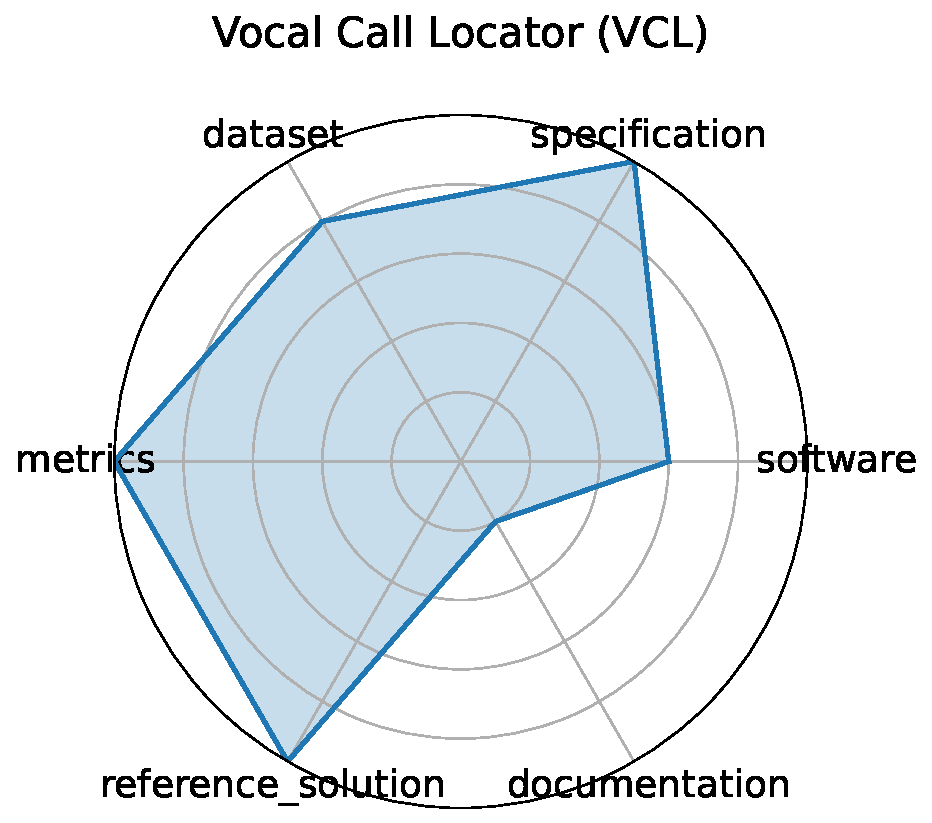
\includegraphics[width=0.2\textwidth]{vocal_call_locator_vcl_radar.pdf}
}}
\clearpage